%%%%%%%%%%%%%%%%%%%%%%%%%%%%%%%%%%%%%%%%%%%%%%%%%%%%%%%%%%%%%%%%%%%%%%
%\fontfamily{cmt}\selectfont
% Template for a UBC-compliant dissertation
% At the minimum, you will need to change the information found
% after the "Document meta-data"
%
%!TEX TS-program = pdflatex
%!TEX encoding = UTF-8 Unicode

%% The ubcdiss class provides several options:
%%   gpscopy (aka fogscopy)
%%       set parameters to exactly how GPS specifies
%%         * single-sided
%%         * page-numbering starts from title page
%%         * the lists of figures and tables have each entry prefixed
%%           with 'Figure' or 'Table'
%%       This can be tested by `\ifgpscopy ... \else ... \fi'
%%   10pt, 11pt, 12pt
%%       set default font size
%%   oneside, twoside
%%       whether to format for single-sided or double-sided printing
%%   balanced
%%       when double-sided, ensure page content is centred
%%       rather than slightly offset (the default)
%%   singlespacing, onehalfspacing, doublespacing
%%       set default inter-line text spacing; the ubcdiss class
%%       provides \textspacing to revert to this configured spacing
%%   draft
%%       disable more intensive processing, such as including
%%       graphics, etc.
%%

% For submission to GPS
\documentclass[gpscopy,onehalfspacing,11pt]{ubcdiss}

% For your own copies (looks nicer)
% \documentclass[balanced,twoside,11pt]{ubcdiss}

%%%%%%%%%%%%%%%%%%%%%%%%%%%%%%%%%%%%%%%%%%%%%%%%%%%%%%%%%%%%%%%%%%%%%%
%%%%%%%%%%%%%%%%%%%%%%%%%%%%%%%%%%%%%%%%%%%%%%%%%%%%%%%%%%%%%%%%%%%%%%
%%
%% FONTS:
%% 
%% The defaults below configures Times Roman for the serif font,
%% Helvetica for the sans serif font, and Courier for the
%% typewriter-style font.  Configuring fonts can be time
%% consuming; we recommend skipping to END FONTS!
%% 
%% If you're feeling brave, have lots of time, and wish to use one
%% your platform's native fonts, see the commented out bits below for
%% XeTeX/XeLaTeX.  This is not for the faint at heart. 
%% (And shouldn't you be writing? :-)
%%

%% NFSS font specification (New Font Selection Scheme)
%\usepackage{times,mathptmx,courier}
%\usepackage[scaled=.92]{helvet}
\renewcommand{\rmdefault}{cmr} % Computer Modern Roman
\renewcommand{\sfdefault}{cmss} % Computer Modern Sans Serif
\renewcommand{\ttdefault}{cmtt} % Computer Modern Typewriter

%% Math or theory people may want to include the handy AMS macros
\usepackage{amssymb}
\usepackage{amsmath}
\usepackage{amsfonts}
\usepackage{prodint}
%% The pifont package provides access to the elements in the dingbat font.   
%% Use \ding{##} for a particular dingbat (see p7 of psnfss2e.pdf)
%%   Useful:
%%     51,52 different forms of a checkmark
%%     54,55,56 different forms of a cross (saltyre)
%%     172-181 are 1-10 in open circle (serif)
%%     182-191 are 1-10 black circle (serif)
%%     192-201 are 1-10 in open circle (sans serif)
%%     202-211 are 1-10 in black circle (sans serif)
%% \begin{dinglist}{##}\item... or dingautolist (which auto-increments)
%% to create a bullet list with the provided character.
\usepackage{pifont}

%%%%%%%%%%%%%%%%%%%%%%%%%%%%%%%%%%%%%%%%%%%%%%%%%%%%%%%%%%%%%%%%%%%%%%
%% Configure fonts for XeTeX / XeLaTeX using the fontspec package.
%% Be sure to check out the fontspec documentation.
%\usepackage{fontspec,xltxtra,xunicode}	% required
%\defaultfontfeatures{Mapping=tex-text}	% recommended
%% Minion Pro and Myriad Pro are shipped with some versions of
%% Adobe Reader.  Adobe representatives have commented that these
%% fonts can be used outside of Adobe Reader.
%\setromanfont[Numbers=OldStyle]{Minion Pro}
%\setsansfont[Numbers=OldStyle,Scale=MatchLowercase]{Myriad Pro}
%\setmonofont[Scale=MatchLowercase]{Andale Mono}

%% Other alternatives:
%\setromanfont[Mapping=tex-text]{Adobe Caslon}
%\setsansfont[Scale=MatchLowercase]{Gill Sans}
%\setsansfont[Scale=MatchLowercase,Mapping=tex-text]{Futura}
%\setmonofont[Scale=MatchLowercase]{Andale Mono}
%\newfontfamily{\SYM}[Scale=0.9]{Zapf Dingbats}
%% END FONTS
%%%%%%%%%%%%%%%%%%%%%%%%%%%%%%%%%%%%%%%%%%%%%%%%%%%%%%%%%%%%%%%%%%%%%%
%%%%%%%%%%%%%%%%%%%%%%%%%%%%%%%%%%%%%%%%%%%%%%%%%%%%%%%%%%%%%%%%%%%%%%



%%%%%%%%%%%%%%%%%%%%%%%%%%%%%%%%%%%%%%%%%%%%%%%%%%%%%%%%%%%%%%%%%%%%%%
%%%%%%%%%%%%%%%%%%%%%%%%%%%%%%%%%%%%%%%%%%%%%%%%%%%%%%%%%%%%%%%%%%%%%%
%%
%% Recommended packages
%%
\usepackage{checkend}	% better error messages on left-open environments
\usepackage{graphicx}	% for incorporating external images

%% booktabs: provides some special commands for typesetting tables as used
%% in excellent journals.  Ignore the examples in the Lamport book!
\usepackage{booktabs}

%% listings: useful support for including source code listings, with
%% optional special keyword formatting.  The \lstset{} causes
%% the text to be typeset in a smaller sans serif font, with
%% proportional spacing.
\usepackage{listings}
\lstset{basicstyle=\sffamily\scriptsize,showstringspaces=false,fontadjust}

%% The acronym package provides support for defining acronyms, providing
%% their expansion when first used, and building glossaries.  See the
%% example in glossary.tex and the example usage throughout the example
%% document.
%% NOTE: to use \MakeTextLowercase in the \acsfont command below,
%%   we *must* use the `nohyperlinks' option -- it causes errors with
%%   hyperref otherwise.  See Section 5.2 in the ``LaTeX 2e for Class
%%   and Package Writers Guide'' (clsguide.pdf) for details.
\usepackage[printonlyused,nohyperlinks]{acronym}
%% The ubcdiss.cls loads the `textcase' package which provides commands
%% for upper-casing and lower-casing text.  The following causes
%% the acronym package to typeset acronyms in small-caps
%% as recommended by Bringhurst.
\renewcommand{\acsfont}[1]{{\scshape \MakeTextLowercase{#1}}}

%% color: add support for expressing colour models.  Grey can be used
%% to great effect to emphasize other parts of a graphic or text.
%% For an excellent set of examples, see Tufte's "Visual Display of
%% Quantitative Information" or "Envisioning Information".
\usepackage{color}
\definecolor{greytext}{gray}{0.5}

%% comment: provides a new {comment} environment: all text inside the
%% environment is ignored.
%%   \begin{comment} ignored text ... \end{comment}
\usepackage{comment}

%% The natbib package provides more sophisticated citing commands
%% such as \citeauthor{} to provide the author names of a work,
%% \citet{} to produce an author-and-reference citation,
%% \citep{} to produce a parenthetical citation.
%% We use \citeeg{} to provide examples
\usepackage[numbers,sort&compress]{natbib}
\newcommand{\citeeg}[1]{\citep[e.g.,][]{#1}}

%% The titlesec package provides commands to vary how chapter and
%% section titles are typeset.  The following uses more compact
%% spacings above and below the title.  The titleformat that follow
%% ensure chapter/section titles are set in singlespace.
\usepackage[compact]{titlesec}
\titleformat*{\section}{\singlespacing\raggedright\bfseries\Large}
\titleformat*{\subsection}{\singlespacing\raggedright\bfseries\large}
\titleformat*{\subsubsection}{\singlespacing\raggedright\bfseries}
\titleformat*{\paragraph}{\singlespacing\raggedright\itshape}

%% The caption package provides support for varying how table and
%% figure captions are typeset.
\usepackage[format=hang,indention=-1cm,labelfont={bf},margin=1em]{caption}

%% url: for typesetting URLs and smart(er) hyphenation.
%% \url{http://...} 
\usepackage{url}
\urlstyle{sf}	% typeset urls in sans-serif


%%%%%%%%%%%%%%%%%%%%%%%%%%%%%%%%%%%%%%%%%%%%%%%%%%%%%%%%%%%%%%%%%%%%%%
%%%%%%%%%%%%%%%%%%%%%%%%%%%%%%%%%%%%%%%%%%%%%%%%%%%%%%%%%%%%%%%%%%%%%%
%%
%% Possibly useful packages: you may need to explicitly install
%% these from CTAN if they aren't part of your distribution;
%% teTeX seems to ship with a smaller base than MikTeX and MacTeX.
%%
%\usepackage{pdfpages}	% insert pages from other PDF files
%\usepackage{longtable}	% provide tables spanning multiple pages
%\usepackage{chngpage}	% support changing the page widths on demand
%\usepackage{tabularx}	% an enhanced tabular environment

%% enumitem: support pausing and resuming enumerate environments.
%\usepackage{enumitem}

%% rotating: provides two environments, sidewaystable and sidewaysfigure,
%% for typesetting tables and figures in landscape mode.  
%\usepackage{rotating}

%% subfig: provides for including subfigures within a figure,
%% and includes being able to separately reference the subfigures.
%\usepackage{subfig}

%% ragged2e: provides several new new commands \Centering, \RaggedLeft,
%% \RaggedRight and \justifying and new environments Center, FlushLeft,
%% FlushRight and justify, which set ragged text and are easily
%% configurable to allow hyphenation.
%\usepackage{ragged2e}

%% The ulem package provides a \sout{} for striking out text and
%% \xout for crossing out text.  The normalem and normalbf are
%% necessary as the package messes with the emphasis and bold fonts
%% otherwise.
%\usepackage[normalem,normalbf]{ulem}    % for \sout

%%%%%%%%%%%%%%%%%%%%%%%%%%%%%%%%%%%%%%%%%%%%%%%%%%%%%%%%%%%%%%%%%%%%%%
%% HYPERREF:
%% The hyperref package provides for embedding hyperlinks into your
%% document.  By default the table of contents, references, citations,
%% and footnotes are hyperlinked.
%%
%% Hyperref provides a very handy command for doing cross-references:
%% \autoref{}.  This is similar to \ref{} and \pageref{} except that
%% it automagically puts in the *type* of reference.  For example,
%% referencing a figure's label will put the text `Figure 3.4'.
%% And the text will be hyperlinked to the appropriate place in the
%% document.
%%
%% Generally hyperref should appear after most other packages

%% The `pagebackref' causes the references in the bibliography to have
%% back-references to the citing page; `backref' puts the citing section
%% number.  See further below for other examples of using hyperref.
%% 2009/12/09: now use `linktocpage' (Jacek Kisynski): GPS now prefers
%%   that the ToC, LoF, LoT place the hyperlink on the page number,
%%   rather than the entry text.
\ifgpscopy
  % GPS requires that weblinks should be dark blue, which looks a bit
  % odd in printed form.
  % https://www.grad.ubc.ca/current-students/dissertation-thesis-preparation/fonts-print
  \usepackage[bookmarks,bookmarksnumbered,%
     pagebackref,linktocpage,%
     colorlinks=true,%
     linkcolor=black,%
     urlcolor=blue,%
     citecolor=black%
     ]{hyperref}
\else
  %% The following puts hyperlinks in very faint grey boxes (in pdf only).
  \usepackage[bookmarks,bookmarksnumbered,%
    pagebackref,linktocpage,%
    allbordercolors={0.8 0.8 0.8},%
    ]{hyperref}
\fi
%% The following change how the the back-references text is typeset in a
%% bibliography when `backref' or `pagebackref' are used
%%
%% Change \nocitations if you'd like some text shown where there
%% are no citations found (e.g., pulled in with \nocite{xxx})
\newcommand{\nocitations}{\relax}
%%\newcommand{\nocitations}{No citations}
%%
%\renewcommand*{\backref}[1]{}% necessary for backref < 1.33
\renewcommand*{\backrefsep}{,~}%
\renewcommand*{\backreftwosep}{,~}% ', and~'
\renewcommand*{\backreflastsep}{,~}% ' and~'
\renewcommand*{\backrefalt}[4]{%
\textcolor{greytext}{\ifcase #1%
\nocitations%
\or
\(\rightarrow\) page #2%
\else
\(\rightarrow\) pages #2%
\fi}}


%% The following uses most defaults, which causes hyperlinks to be
%% surrounded by colourful boxes; the colours are only visible in
%% PDFs and don't show up when printed:
%\usepackage[bookmarks,bookmarksnumbered]{hyperref}

%% The following disables the colourful boxes around hyperlinks.
%\usepackage[bookmarks,bookmarksnumbered,pdfborder={0 0 0}]{hyperref}

%% The following disables all hyperlinking, but still enabled use of
%% \autoref{}
%\usepackage[draft]{hyperref}

%% The following commands causes chapter and section references to
%% uppercase the part name.
\renewcommand{\chapterautorefname}{Chapter}
\renewcommand{\sectionautorefname}{Section}
\renewcommand{\subsectionautorefname}{Section}
\renewcommand{\subsubsectionautorefname}{Section}

%% If you have long page numbers (e.g., roman numbers in the 
%% preliminary pages for page 28 = xxviii), you might need to
%% uncomment the following and tweak the \@pnumwidth length
%% (default: 1.55em).  See the tocloft documentation at
%% http://www.ctan.org/tex-archive/macros/latex/contrib/tocloft/
% \makeatletter
% \renewcommand{\@pnumwidth}{3em}
% \makeatother

%%%%%%%%%%%%%%%%%%%%%%%%%%%%%%%%%%%%%%%%%%%%%%%%%%%%%%%%%%%%%%%%%%%%%%
%%%%%%%%%%%%%%%%%%%%%%%%%%%%%%%%%%%%%%%%%%%%%%%%%%%%%%%%%%%%%%%%%%%%%%
%%
%% Some special settings that controls how text is typeset
%%
% \raggedbottom		% pages don't have to line up nicely on the last line
% \sloppy		% be a bit more relaxed in inter-word spacing
% \clubpenalty=10000	% try harder to avoid orphans
% \widowpenalty=10000	% try harder to avoid widows
% \tolerance=1000

%% And include some of our own useful macros
% This file provides examples of some useful macros for typesetting
% dissertations.  None of the macros defined here are necessary beyond
% for the template documentation, so feel free to change, remove, and add
% your own definitions.
%
% We recommend that you define macros to separate the semantics
% of the things you write from how they are presented.  For example,
% you'll see definitions below for a macro \file{}: by using
% \file{} consistently in the text, we can change how filenames
% are typeset simply by changing the definition of \file{} in
% this file.
% 
%% The following is a directive for TeXShop to indicate the main file
%%!TEX root = diss.tex

\newcommand{\NA}{\textsc{n/a}}	% for "not applicable"
\newcommand{\eg}{e.g.,\ }	% proper form of examples (\eg a, b, c)
\newcommand{\ie}{i.e.,\ }	% proper form for that is (\ie a, b, c)
\newcommand{\etal}{\emph{et al}}

% Some useful macros for typesetting terms.
\newcommand{\file}[1]{\texttt{#1}}
\newcommand{\class}[1]{\texttt{#1}}
\newcommand{\latexpackage}[1]{\href{http://www.ctan.org/macros/latex/contrib/#1}{\texttt{#1}}}
\newcommand{\latexmiscpackage}[1]{\href{http://www.ctan.org/macros/latex/contrib/misc/#1.sty}{\texttt{#1}}}
\newcommand{\env}[1]{\texttt{#1}}
\newcommand{\BibTeX}{Bib\TeX}

% Define a command \doi{} to typeset a digital object identifier (DOI).
% Note: if the following definition raise an error, then you likely
% have an ancient version of url.sty.  Either find a more recent version
% (3.1 or later work fine) and simply copy it into this directory,  or
% comment out the following two lines and uncomment the third.
\DeclareUrlCommand\DOI{}
\newcommand{\doi}[1]{\href{http://dx.doi.org/#1}{\DOI{doi:#1}}}
%\newcommand{\doi}[1]{\href{http://dx.doi.org/#1}{doi:#1}}

% Useful macro to reference an online document with a hyperlink
% as well with the URL explicitly listed in a footnote
% #1: the URL
% #2: the anchoring text
\newcommand{\webref}[2]{\href{#1}{#2}\footnote{\url{#1}}}

% epigraph is a nice environment for typesetting quotations
\makeatletter
\newenvironment{epigraph}{%
	\begin{flushright}
	\begin{minipage}{\columnwidth-0.75in}
	\begin{flushright}
	\@ifundefined{singlespacing}{}{\singlespacing}%
    }{
	\end{flushright}
	\end{minipage}
	\end{flushright}}
\makeatother

% \FIXME{} is a useful macro for noting things needing to be changed.
% The following definition will also output a warning to the console
\newcommand{\FIXME}[1]{\typeout{**FIXME** #1}\textbf{[FIXME: #1]}}

% END


%%%%%%%%%%%%%%%%%%%%%%%%%%%%%%%%%%%%%%%%%%%%%%%%%%%%%%%%%%%%%%%%%%%%%%
%%%%%%%%%%%%%%%%%%%%%%%%%%%%%%%%%%%%%%%%%%%%%%%%%%%%%%%%%%%%%%%%%%%%%%
%%
%% Document meta-data: be sure to also change the \hypersetup information
%%

\title{Penalized Competing Risks Analysis using Case-Base Sampling for High-Dimensional Data}
%\subtitle{If you want a subtitle}

\author{Nirupama Tamvada}
\previousdegree{B.Sc, 2021}

% What is this dissertation for?
\degreetitle{Master of Science}

\institution{The University of British Columbia}
\campus{Vancouver}

\faculty{The Faculty of Graduate and Postdoctoral Studies}
\department{Statistics}
\submissionmonth{August}
\submissionyear{2023}

% details of your examining committee
\examiningcommittee{Gabriela V. Cohen Freue, Associate Professor, Statistics, \textsc{UBC}}{Supervisor}
\examiningcommittee{Paul Gustafson, Professor, Statistics, \textsc{UBC}}{Supervisory Committee Member}

%% hyperref package provides support for embedding meta-data in .PDF
%% files
\hypersetup{
  pdftitle={Change this title!  (DRAFT: \today)},
  pdfauthor={Johnny Canuck},
  pdfkeywords={Your keywords here}
}

%%%%%%%%%%%%%%%%%%%%%%%%%%%%%%%%%%%%%%%%%%%%%%%%%%%%%%%%%%%%%%%%%%%%%%
%%%%%%%%%%%%%%%%%%%%%%%%%%%%%%%%%%%%%%%%%%%%%%%%%%%%%%%%%%%%%%%%%%%%%%
%% 
%% The document content
%%

%% LaTeX's \includeonly commands causes any uses of \include{} to only
%% include files that are in the list.  This is helpful to produce
%% subsets of your thesis (e.g., for committee members who want to see
%% the dissertation chapter by chapter).  It also saves time by 
%% avoiding reprocessing the entire file.
%\includeonly{intro,co nclusions}
%\includeonly{discussion}

\begin{document}

%%%%%%%%%%%%%%%%%%%%%%%%%%%%%%%%%%%%%%%%%%%%%%%%%%
%% From Thesis Components: Tradtional Thesis
%% <http://www.grad.ubc.ca/current-students/dissertation-thesis-preparation/order-components>
%\fontfamily{cmt}\selectfont
% Preliminary Pages (numbered in lower case Roman numerals)
%    1. Title page (mandatory)
\maketitle
%    2. Committee page (mandatory): lists supervisory committee and,
%    if applicable, the examining committee
\makecommitteepage

%    3. Abstract (mandatory - maximum 350 words)
%% The following is a directive for TeXShop to indicate the main file
%%!TEX root = diss.tex

\chapter{Abstract}

This document provides brief instructions for using the \class{ubcdiss}
class to write a \acs{UBC}-conformant dissertation in \LaTeX.  This
document is itself written using the \class{ubcdiss} class and is
intended to serve as an example of writing a dissertation in \LaTeX.
This document has embedded \acp{URL} and is intended to be viewed
using a computer-based \ac{PDF} reader.

Note: Abstracts should generally try to avoid using acronyms.

Note: at \ac{UBC}, both the \ac{GPS} Ph.D. defence programme and the
Library's online submission system restricts abstracts to 350
words.

\ifgpscopy
  This document was typeset in \texttt{gpscopy} mode.
\else
  This document was typeset in non-\texttt{gpscopy} mode.
\fi

% Consider placing version information if you circulate multiple drafts
%\vfill
%\begin{center}
%\begin{sf}
%\fbox{Revision: \today}
%\end{sf}
%\end{center}

\cleardoublepage

%    4. Lay Summary (Effective May 2017, mandatory - maximum 150 words)
%% The following is a directive for TeXShop to indicate the main file
%%!TEX root = diss.tex

%% https://www.grad.ubc.ca/current-students/dissertation-thesis-preparation/preliminary-pages
%% 
%% LAY SUMMARY Effective May 2017, all theses and dissertations must
%% include a lay summary.  The lay or public summary explains the key
%% goals and contributions of the research/scholarly work in terms that
%% can be understood by the general public. It must not exceed 150
%% words in length.

\chapter{Lay Summary}

High-dimensional genomic data to correlate is commonly generated currently 
\cleardoublepage

%    5. Preface
%% The following is a directive for TeXShop to indicate the main file
%%!TEX root = diss.tex

\chapter{Preface}

This thesis is original, unpublished work by the author under the supervision of Prof. Gabriela V. Cohen Freue. This thesis is a collaborative product with the CANSII-CRT research group. The research topic was proposed by Prof. Gabriela V. Cohen Freue, in collaboration with Dr. Sahir Bhatnagar, and Dr. Maxime Turgeon. The casebase framework was proposed by Dr. James A. Hanley and Dr. Olli S. Miettinen, and the software was implemented by Dr. Sahir Bhatnagar and Dr. Maxime Turgeon. The optimization for the penalized multinomial regression model used is not currently part of the \texttt{casebase} package and was written by Dr. Yi Lian, with modifications made by the author to correctly fit the penalty functions. The author also solely contributed additional functions for the fitting of the penalized model. All empirical studies and the data analysis were designed and carried out by the author in discussion with Prof. Gabriela V. Cohen Freue. All text and code for the experiments in the thesis were written by the author, aside from the use of \texttt{R} packages that were developed by other authors and obtained from the Comprehensive \texttt{R} Archived Network (CRAN).
\cleardoublepage

%    6. Table of contents (mandatory - list all items in the preliminary pages
%    starting with the abstract, followed by chapter headings and
%    subheadings, bibliographies and appendices)
\tableofcontents
\cleardoublepage	% required by tocloft package

%    7. List of tables (mandatory if thesis has tables)
\listoftables
\cleardoublepage	% required by tocloft package

%    8. List of figures (mandatory if thesis has figures)
\listoffigures
\cleardoublepage	% required by tocloft package

%    9. List of illustrations (mandatory if thesis has illustrations)
%   10. Lists of symbols, abbreviations or other (optional)

%   11. Glossary (optional)
%%% The following is a directive for TeXShop to indicate the main file
%%!TEX root = diss.tex

\chapter{Glossary}

This glossary uses the handy \latexpackage{acroynym} package to automatically
maintain the glossary.  It uses the package's \texttt{printonlyused}
option to include only those acronyms explicitly referenced in the
\LaTeX\ source.  To change how the acronyms are rendered, change the
\verb+\acsfont+ definition in \verb+diss.tex+.

% use \acrodef to define an acronym, but no listing
\acrodef{UI}{user interface}
\acrodef{UBC}{University of British Columbia}

% The acronym environment will typeset only those acronyms that were
% *actually used* in the course of the document
\begin{acronym}[ANOVA]
\acro{ANOVA}[ANOVA]{Analysis of Variance\acroextra{, a set of
  statistical techniques to identify sources of variability between groups}}
\acro{API}{application programming interface}
\acro{CTAN}{\acroextra{The }Common \TeX\ Archive Network}
\acro{DOI}{Document Object Identifier\acroextra{ (see
    \url{http://doi.org})}}
\acro{GPS}[GPS]{Graduate and Postdoctoral Studies}
\acro{PDF}{Portable Document Format}
\acro{RCS}[RCS]{Revision control system\acroextra{, a software
    tool for tracking changes to a set of files}}
\acro{TLX}[TLX]{Task Load Index\acroextra{, an instrument for gauging
  the subjective mental workload experienced by a human in performing
  a task}}
\acro{UML}{Unified Modelling Language\acroextra{, a visual language
    for modelling the structure of software artefacts}}
\acro{URL}{Unique Resource Locator\acroextra{, used to describe a
    means for obtaining some resource on the world wide web}}
\acro{W3C}[W3C]{\acroextra{the }World Wide Web Consortium\acroextra{,
    the standards body for web technologies}}
\acro{XML}{Extensible Markup Language}
\end{acronym}

% You can also use \newacro{}{} to only define acronyms
% but without explictly creating a glossary
% 
% \newacro{ANOVA}[ANOVA]{Analysis of Variance\acroextra{, a set of
%   statistical techniques to identify sources of variability between groups.}}
% \newacro{API}[API]{application programming interface}
% \newacro{GOMS}[GOMS]{Goals, Operators, Methods, and Selection\acroextra{,
%   a framework for usability analysis.}}
% \newacro{TLX}[TLX]{Task Load Index\acroextra{, an instrument for gauging
%   the subjective mental workload experienced by a human in performing
%   a task.}}
% \newacro{UI}[UI]{user interface}
% \newacro{UML}[UML]{Unified Modelling Language}
% \newacro{W3C}[W3C]{World Wide Web Consortium}
% \newacro{XML}[XML]{Extensible Markup Language}
	% always input, since other macros may rely on it

\textspacing		% begin one-half or double spacing

%   12. Acknowledgements (optional)
%% The following is a directive for TeXShop to indicate the main file
%%!TEX root = diss.tex

\chapter{Acknowledgments}

First and foremost, I would like to acknowledge my supervisor, Prof. Gabriela V. Cohen Freue, for her valuable support and insightful feedback throughout my M.Sc. I am also thankful to Prof. Paul Gustafson for taking the time to read and evaluate my thesis. I would also like to thank Dr. Yi Lian for his helpful advice. I am also very thankful to Dr. Sahir Bhatnagar, Dr. Maxime Turgeon and to the whole CANSII CRT group, for the fruitful collaboration on \texttt{casebase}, and for the financial support through my MSc. Additionally, I want to thank Maxwell Douglas, Evan Popoff and Basia Rogula for their support during my co-op work terms. I also wish to extend my sincere gratitude to my undergraduate supervisor Dr. Ian Dworkin, who actively gave me the confidence and encouragement to pursue grad school and research.
\bigskip \par
I am grateful for all of my wonderful fellow classmates and friends both in and outside the Department of Statistics. I want to thank Caitlin, Mansi, and Sangay in particular for the many good times. I also wish to acknowledge my fellow lab members, Chloe, Giuseppe, Maggie, and Jana, in particular for coding and writing along with me everyday in Koerner. I would also like to thank Dr. Anthony Christidis for his helpful advice on my simulations. I am very grateful to the Department of Statistics for their prompt support and help, and for their financial support through the Rick White Award. I also want to thank Alex Romanus for contributing to my project as a part of his USRA.
\bigskip \par
Finally, I am thankful for my family. I would not have been able to accomplish any of this without their love and support.

\bigskip \par




%   13. Dedication (optional)

% Body of Thesis (not all sections may apply)
\mainmatter

\acresetall	% reset all acronyms used so far

%    1. Introduction
 %% The following is a directive for TeXShop to indicate the main file
%%!TEX root = diss.tex

\chapter{Introduction}
\label{ch:Introduction}

\begin{flushleft}
%\begin{epigraph}
    \textbf{Reid:} How do you feel about the cottage industry that’s grown up around it [the Cox model]?
    \\
\textbf{Cox:} Don’t know, really. In the light of some of the further results one knows since, I think I would normally want to tackle problems parametrically, so I would take the underlying hazard to be a Weibull or something. I’m not keen on nonparametric formulations usually.
\\
\textbf{Reid:} So if you had a set of censored survival data today, you might rather fit a parametric model, even though there was a feeling among the medical statisticians that that wasn’t quite right.
\\
\textbf{Cox:} That’s right, but since then various people have shown that the answers are very insensitive to the parametric formulation of the underlying distribution [see, e.g., Cox and Oakes, Analysis of Survival Data, Chapter 8.5]. And if you want to do things like predict the outcome for a particular patient, it’s much more convenient to do that parametrically.

- \textit{Sir. David Cox's reflections on the semi-parametric proportional hazards model (Reid, 1994)}
%\end{epigraph}
\end{flushleft}

In many clinical studies, the main outcome that is being modelled is the time to an event of interest or the \textit{survival} time within the study time period. If the event is experienced by all the individuals in a study, many methods of statistical analyses would be applicable. However, some of the difficulties faced in analyzing survival data are as follows: 1) not all the patients experience the event of interest within the study period (but are still at \textit{risk} to do so in the future). Thus, their true time to the event of interest is unknown. 2) survival data are rarely normally distributed and generally have a skewed shape. For these reasons, the development of methods tailored in particular to \textit{survival data} are necessary. Typically, in the analysis of survival or time-to-event data, we analyze data where the outcome variable denotes the time to occurrence of one event of interest. Often, however, a combined endpoint is a common extension of typical survival analysis, that is, a having cause of interest and a competing risk.  In this context, a competing risk is an event whose occurrence precludes the occurrence of the primary event of interest. For instance, medical studies often consider ‘disease-free survival’, i.e., time until (recurrence of a) disease or death (without prior disease), whichever comes first. In this scenario, while death due to prior disease is our primary cause of interest, death without prior disease (of another cause) would be considered a competing risk.
\medskip \par
From a clinical view-point, the most important quantity of interest from a survival analysis to both clinicians and patients is an estimate of the risk of an event to a patient, given a particular covariate profile. This risk can be obtained by estimating the cumulative incidence function (CIF) (also known as the absolute risk), which is the probability that a person at risk will experience the event of interest within a specified time-interval. One of the most widely used methods that has been developed for the survival analysis of a single-endpoint is the Cox Proportional Hazards model. The flexibility of this model comes from its semi-parametric formulation, which enables the convenient inference of the influence of the covariates on the hazard function, without restraining the response to a particular parametric family. However, this flexibility comes at a cost: the baseline hazard is de-coupled from the effect of the covariates. Thus, the baseline hazard needs to be estimated separately for calculating the cumulative incidence function. This results in step-wise estimates of survival risk, which are often difficult to interpret. Additionally, extending the cox proportional hazards model to the competing risks scenario would involve fitting a cox proportional hazards model for each of the competing risks. This approach is limited by the fact that while the cause-specific hazards can estimated, we cannot estimate the \textit{cumulative incidence} of the event of the interest while simultaneously accounting for competing risks. For this reason, the Fine-Gray model was proposed as an alternative, as this approach directly models the effect of the covariates on the cumulative incidence function. However, when interested in whether a given risk factor or characteristic is associated with the rate of the occurrence of the outcome in subjects who are currently event‐free, we would be interested in the cause-specific hazards as well, which in this model would not be easily available. Furthermore, with certain combinations of covariates, the Fine-Gray model often gives estimates of the cumulative incidence probability that exceed 1 (which we additionally demonstrate here). Indeed, in modelling competing risks, all the available approaches either model the cause-specific hazards or the cumulative incidence function, and while a complete competing risks survival analysis requires both, the process to estimate the other is not quite straight-forward in the currently available models. The generation of survival data, particularly high-dimensional data is becoming more commonplace, and thus, we are in need of a competing risks model that can model the cause-specific hazards, generate an easily interpretable smooth estimate of the cumulative incidence function, and builds a general framework that can be easily extended to applications such as variable selection in high-dimensional data, as well as situations such as time-varying covariates. Thus, in this thesis, we propose to use a multinomial model in combination with \textit{casebase sampling} to fit fully parametric hazard models. This approach comes with the benefits of generating smooth-in-time hazard and cumulative incidence functions. Furthermore, our use of the multinomial regression means that we have access to the nice properties of the generalized linear models family, including variable selection through regularization. In this thesis, we show that the multinomial model with casebase sampling offers good variable selection performance, in both low and high-dimensional data, and additionally shows good performance in predicting the cumulative risk, making this model a viable option for performing a complete competing risks analysis. This thesis is organized as follows: in chapter 2, we give a detailed background of competing risks survival analysis and the currently existing approaches for this kind of data. In chapter 3, we then discuss the mathematical and computational details of the casebase multinomial implementation. In chapter 4, we discuss the results of our simulation experiments, looking at the variable selection, prediction performance, as well as looking into two case-studies, which highlight desirable properties of casebase in relation to other competitors. Finally we conclude this thesis in chapter 5 with mentions of some limitations and extensions of the approach and the simulations performed for future work. 

 

\chapter{Background}
\label{ch:Background}

In this chapter, we give a broad overview of survival analysis and extend a single end-point survival analysis to a competing risks scenario. We then discuss the two broad classes of approaches used to model competing risks and subsequently motivate the penalized casebase multinomial model. We also include a summary of regularized methods to perform variable selection for competing risks. Finally, we conclude the chapter by discussing the some metrics used to quantify the performance of survival analysis models, which motivate our experiments in Chapter 4. The notation defined in this section is used throughout this work.


\section{Survival Analysis}

We consider a simple multistate model to understand survival analysis, as depicted in \autoref{fig:fig1}. Each individual in the study starts at the initial stage of 0. At some time $T$, the individual moves to the absorbing state 1 which represents the event of interest. Our outcome of interest is this time to event $T$, also known as the survival time. 


\begin{figure}[h]
    \centering
    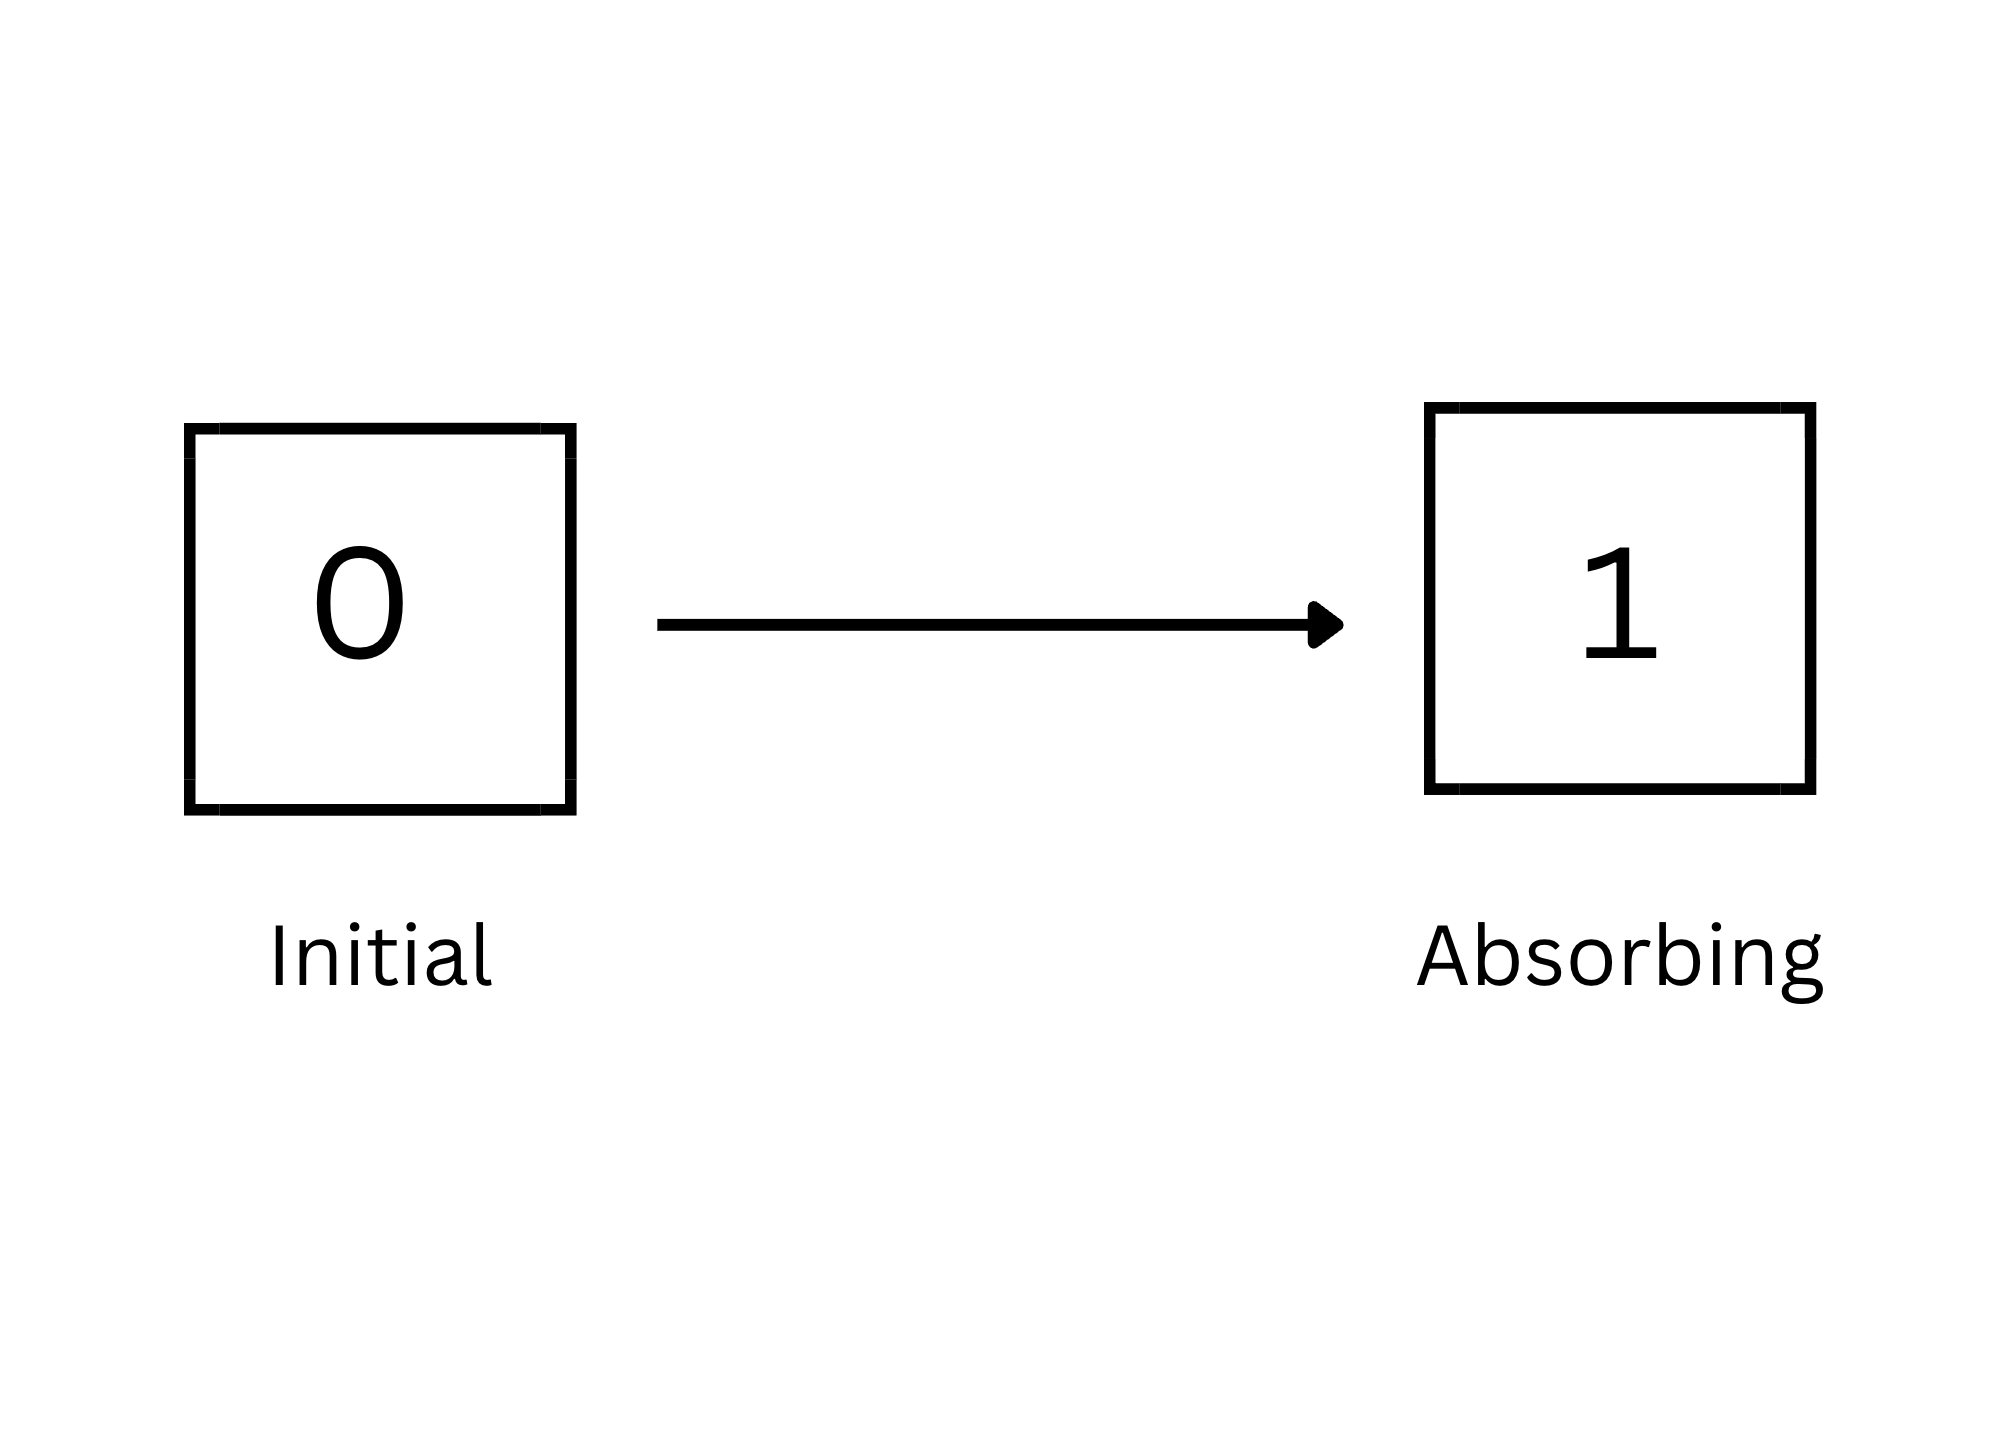
\includegraphics[width=3in]{survival_mstate.png}
    \caption{Single end-point survival analysis represented through a multi-state model}
    \label{fig:fig1}   % label should change
    \end{figure}

In our inference of $T$, we record the state $X_{T}$ at which an individual is at every point of time $t \geq 0$, $X_T \in \{0, 1 \}$. As long as the individual is in the initial stage of 0, they are considered at \textit{risk} to transition to 1. Our time-to event is then the smallest time $T$ at which the individual is no longer in stage 0, i.e. $T := \textrm{inf}\{t : X_{T} \neq 0 \}$. Recording of an individual will stop once the individual has reached the absorbing state 1.
\bigskip \par
Survival analysis has evolved from its initial focus on modeling time to death as the primary event of interest to encompass a wide range of events in various fields of study. Today, it is extensively employed in modeling events such as the time till the onset of disease, time till employment, stock market crashes, earthquakes, and more. In the clinical and biomedical field, time-to-event data remains particularly prevalent and invaluable due to its ability to provide crucial insights into the prognosis and survival outcomes of patients. The development of accurate methods for survival analysis enables researchers and healthcare professionals to effectively assess the effectiveness of interventions and treatments. By incorporating the temporal perspective, survival analysis plays a critical role in understanding the evolving nature of diseases and treatments, allowing for the evaluation of long-term patient outcomes, such as the 5-year risk of disease onset or the probability of patient survival. These insights are essential for guiding clinical decision-making and tailoring treatment strategies to individual patients.
\bigskip \par
Furthermore, survival analysis provides a valuable tool for identifying prognostic factors or covariates that significantly influence survival. By quantifying the effects of specific genetic biomarkers, demographic factors, or treatment modalities, researchers can gain a deeper understanding of the underlying mechanisms that impact disease progression and patient outcomes. This knowledge empowers additionally guides clinical decision-making, as clinicians can further tailor their approach based on the unique characteristics and circumstances of each patient. 
\bigskip \par
In the subsequent sections, we  delve into the details of survival analysis techniques. Additionally, we will discuss how these techniques facilitate the identification of prognostic factors, as well as the quantification of long-term clinical patient outcomes. 

\subsection{Censoring}

A challenging and unique aspect of survival analysis data is censoring. We describe an individual as censored when an observation does not have an exact survival time. There are many reasons that an individual could end up censored in a study, including study drop out, survival up until the end of the study, or for some reason due to which their precise failure time is not observed. 

There are different types of censoring scenarios that could occur, which include left censoring, interval censoring, and right censoring, among which the latter is the most common. Right censoring occurs typically when either 1) an individual experiences the event of interest after the study period, 2) an individual is withdrawn from the study or 3) a subject is lost to follow-up. In this work, we will only consider the scenario of right-censoring, and hence, omit discussion of other censoring schemes. As right-censoring is the most common scheme, there are methods designed specifically for this kind of data, which deal with three categories of right-censored data: Type I, Type II and Type III censoring. 
\smallskip \par
In Type I censoring (which we depict in \autoref{fig:fig2}), we consider the scenario where a study starts with a fixed number of subjects, all of whom have the beginning of the study as the starting point of their observation period. If an individual is lost to follow up, survives till the end of the study, or is withdrawn from the study, their survival time is censored. The survival time is recorded for all other individuals whose time-to-event falls within the study time-period. In this work, we consider Type-I censoring for simplicity and thus, will define the casebase framework under this scenario as well (although it can be extended generally to other censoring scenarios as well). 
\smallskip \par
However, it should be noted that for many survival studies, a common occurrence is Type III censoring, where a study period starts and ends at fixed times, but individuals may enter the study at any time. If we consider two individuals who do not experience the event of interest until the end of the study, unlike Type I censoring, these two individuals will not have the same censoring time, as the two individuals start the study at different times, which needs to be accounted for. 
\smallskip \par
The general takeaway is that censoring complicates the analysis of survival data. The time we actually observe through a survival study can be constructed as $\tilde{T}$ = $(T \wedge C, \textbf{1}(T \leq C))$ i.e the minimum of the event time $T$ and the censoring time $C$. This needs to be addressed carefully by any method proposed for survival analysis.

\begin{figure}[h]
    \centering
    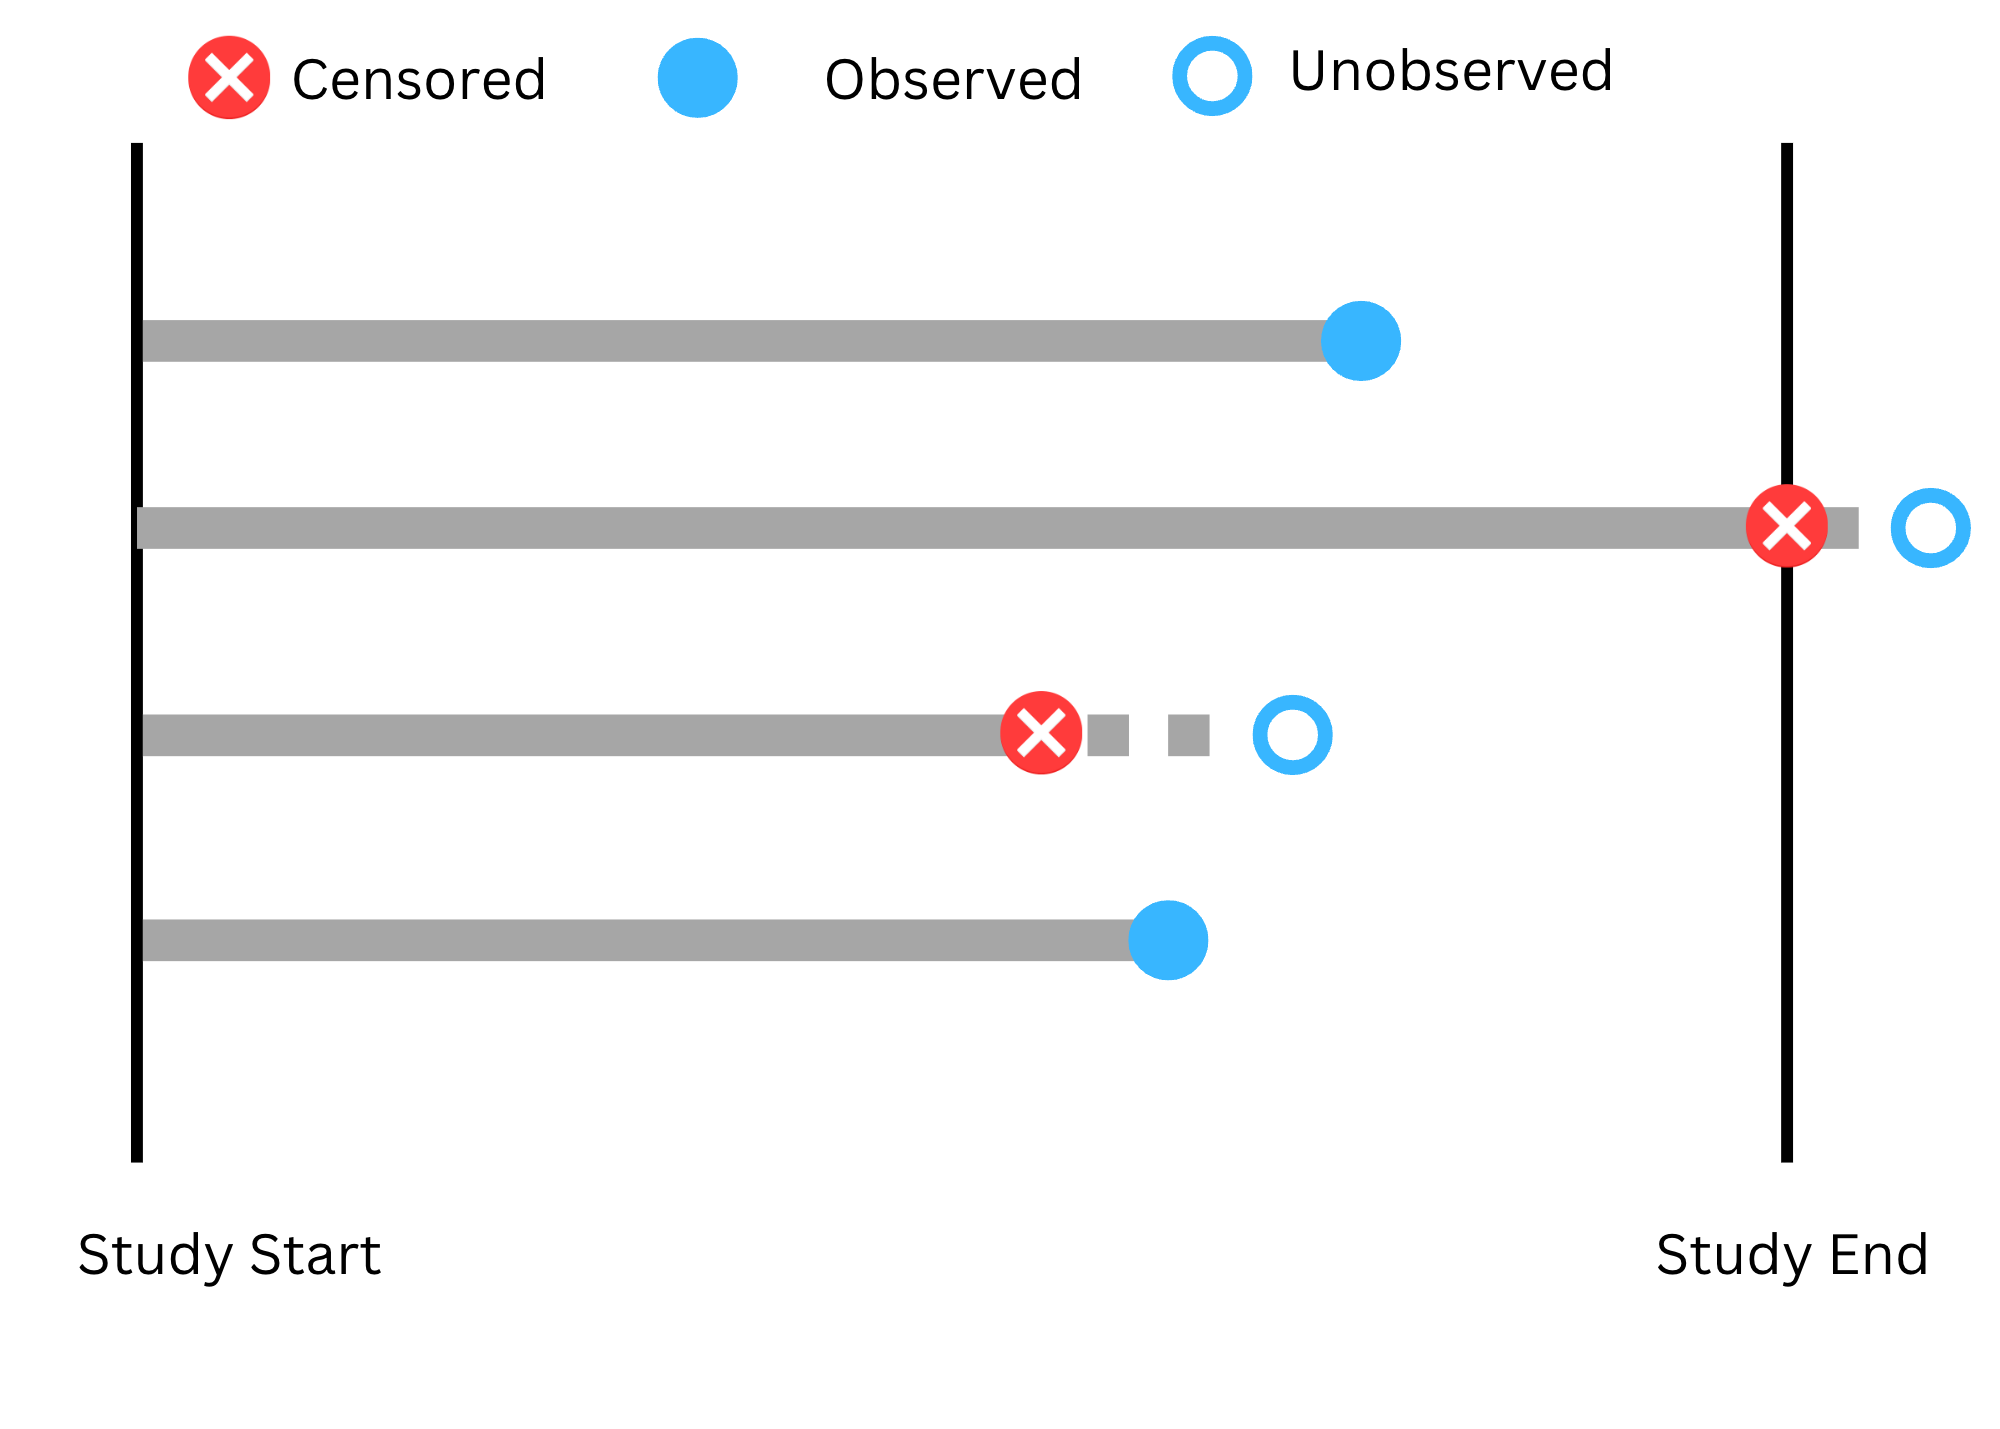
\includegraphics[width=3in]{censoring.png}
    \caption{Schematic of Type I right-censoring. Individual 2 is lost to follow-up and Individual 4 experienced the event after the end of the study, thus both are censored.}
    \label{fig:fig2}   % label should change
    \end{figure}

\subsection{Hazard function}

Typically in a survival analysis, we relate the distribution of $T$ to the covariates of interest by using the hazard function $\alpha(t)$. The hazard can be interpreted as the probability that an individual at risk at time $t$ has an event in time $dt$. Intuitively, the hazard can be interpreted as a rate: specifically the represents the instantaneous event rate for an individual who has already survived to time $t$. The hazard can thus be expressed as: 
\begin{equation}
\alpha(t) \cdot dt := \lim_{\Delta t \searrow 0} \frac{P(T \in [t, t + \Delta t)| T \geq t)}{\Delta t}
\end{equation}

The primary reason that survival analysis methods are hazard-based is due to censoring. As the censoring time $C$ and event $T$ are considered independent, the probability that the event occurs in $dt$ conditional on $T \wedge C \geq t$ is the same as in the absence of censoring, that is:
\begin{equation}
\alpha(t) \cdot dt := \mathbb{P}(T \in dt| T \geq t) = P(T \in dt, T \leq C|T \wedge C \geq t)
\end{equation}

This enables the estimation of the distribution function of $T$ (which we will elaborate on below) even in the presence of censoring, as well as the convenient extension of such hazard-based methods to the competing risks scenario. The intuitive rate interpretation also adds to the advantages of a hazard-based survival analysis approach.

\subsection{The survival function and its relationship to the cumulative hazard}

The distribution function of the event time $T$ can be recovered from the cumulative hazard $A(t)$ as such: 

\begin{equation}
F(t) := 1 - S(t) := P(T \leq t) = 1 - \textrm{exp}(-A(t))
\end{equation}

where $A(t)$ represents the cumulative hazard function $A(t) := \int_{0}^{t} \alpha(u) du$, which provides a measure of the cumulative risk of experiencing an event up to a specific time point. Here, $S(t)$ is referred to as the survival probability. This probability is complementary to the cumulative distribution function $F(t)$, and can be interpreted as the probability that an individual survives longer/is event-free than some specified time \textbf{t}. This probability is often of interest from the perspective of clinical patient care, as the most relevant quantity is often estimating the long-term risk of experiencing a certain event given the patient’s particular characteristics.
\smallskip \par

When analyzing time-to-event data, The Kaplan-Meier estimator is a commonly used non-parametric method for estimating the survival function $S(t)$.
Through this estimator, the survival function can be expressed as a product integral of the cumulative hazards over time $t$ as such: 
\begin{equation}
S(t) = \Prodi_{0}^{t} (1- d\hat{A}(u)) \approx \prod_{k = 1}^{K} (1- \Delta \hat{A}(t_k)) \approx \prod_{k = 1}^{K} P(T > t_k | T > t_{k-1})
\end{equation}

where the ordered sequence of observed event times $0 = t_0 < t_1 < t_2 <...< t_{K-1} <t_K$ partitions the time interval $[0,t]$. The cumulative hazard $\hat{A}(t_k)$ is represented by the Nelson-Aalen estimator here, which can be written as:
\begin{equation}
\hat{A}(t_k) = \frac{\text{Number of individuals \textit{observed} to fail at $t_k$}}{\text{Number of individuals \textit{at risk} just prior to $t_k$}}
\end{equation}


The Kaplan-Meier estimator provides a stepwise estimate of the survival function by taking into account the observed event times and censoring information. The Nelson-Aalen estimator is also non-parametric method, which estimates the cumulative hazard function $A(t)$ directly from the observed event times. It takes into account both the observed events and the associated event times, without assuming any specific distribution for the hazard function. Both the Kaplan-Meier estimator and the Nelson-Aalen estimator are valuable tools in a single-end point survival analysis, allowing researchers to estimate the survival function and the cumulative hazard function, respectively. These estimators provide valuable clinical insights into the survival experience and cumulative risk of experiencing an event over time, even in the presence of censored data. It is important to note the connection back to the hazard function here, namely that the accurate estimation of the cumulative hazard plays an essential role in estimating the survival function.


\section{Cox-Proportional Hazards Model}

Survival analysis has been greatly shaped over the last few decades by the partial likelihood approach of the Cox proportional hazard model. The Cox Proportional Hazards model specifies that the conditional hazard function of failure time given a set of covariates is the product of an unknown baseline hazard function and an exponential regression function of covariates of the form:
\begin{equation}
\lambda(t|X_i) = e^{\beta^T X_i(t)} \lambda_0 (t)
\end{equation}

Here, $X_i = (X_{i1}, … , X_{ip})$ represent the realized values of the covariates for subject $i$, $\lambda(t|X_i)$ represents the  hazard function at time $t$ for subject $i$ with covariate vector $X_i$, $\beta$ represents an unknown set of regression parameters. 
\smallskip\par
Note that the baseline hazard between subjects is identical ($\lambda_0 (t)$) with no dependency on $i$. This is connected to the "proportional" aspect of the Cox model, i.e. its assumption that the hazards for any two individuals have the same proportion at all times, which can be shown as below:
\begin{equation}
\frac{\lambda(t|X_2)}{\lambda(t|X_2)} = \frac{\lambda_0 (t) \dot e^{\beta_2^T X_1(t)}}{\lambda_0 (t) \dot e^{\beta_1^T X_2(t)}} = \frac{e^{\beta_2^T X_1(t)}}{e^{\beta_1^T X_2(t)}}
\end{equation}

i.e the only difference between subjects' hazards comes from the baseline scaling factor $e^{\beta^T X_i(t)}$. In a Cox proportional hazards regression model, the measure in relation to which the regression coefficients are quantified is the hazard rate. In etiological studies, it is often of interest to assess the association between several risk factors and survival time, and interpretation in terms of the hazard is often ideal for this type of analysis. For example, we can easily make interpretations such as a 1-unit change in Age can increase the rate of occurrence of event by 2.11 with the coefficients estimated by a Cox-Proportional Hazards model. The hazard ratios estimated by the Cox model are among those individuals who are actually at risk of developing the event of interest i.e. ‘among those patients who did not (yet) experience the event of interest or a competing event’. As such, this hazard-based modelling approach has the advantage of being easily interpretable for clinicians in studies where the aim of interest is to quantify the effect of prognostic risk factors/covariates in relation to survival time for the \textit{risk set} of patients. 
\smallskip\par
Note that in the estimation of a Cox Proportional Hazards model, the baseline hazard $\lambda_0 (t)$ is treated as a nuisance parameter, and is not estimated with the coefficients. Thus, the cumulative baseline-hazard function needs to be separately estimated. However, the cumulative baseline-hazard is an essential quantity to estimate the survival function. To this end, the Breslow estimator, which extends the Nelson-Aalen estimator to the Cox model with coefficients was proposed to estimate the baseline cumulative hazard function for a Cox model, which takes the form: 
\begin{equation}
\hat{A}_0(t) = \sum_{i =1}^{n} \frac{I(\tilde{T_i} \leq t) \Delta_i}{\sum_{i \in \mathcal{R}_i} \exp(\hat{\beta}^T \mathbf{X}_i(\tilde{T_i}))}
\end{equation}

where  $\tilde{T}$ = $(T \wedge C, \textbf{1}(T \leq C))$, $I(.)$ represents the indicator function, and $\Delta_i$ represents the numerator of the Nelson-Aalen estimator, i.e the number of individuals \textit{observed} to fail at $t$. The conditional survival function under $X = x$ can then be estimated from the Cox model as such:
\begin{equation}
\hat{S}(t) = \exp \left\{ - \int_{0}^{t} exp(\hat{\beta}^T x(u)) d\hat{A}(u) \right\}
\end{equation}

The conditional survival survival function with the Breslow estimator provides a more accurate approximation than the Kaplan-Meier estimator by assigning equal weight to all individuals at risk within each interval. The Breslow estimator comes with the advantage of being non-parametric and not assuming a specific form for the hazard, as its estimation process is based on summing up the number of events at each time-point. However, this comes at a cost of estimating a step-wise survival function (depicted in \autoref{fig:fig3}). As a result of the estimation process, the step-wise Breslow estimate exhibits sudden changes or jumps at the observed event times. These jumps can make it challenging to visually interpret the estimated survival function, especially in small samples, when there are a limited number of observed event times or when the event times are irregularly spaced. The jumps in the estimated survival function can give the impression of abrupt changes in survival probabilities, even when the underlying true survival function may exhibit a smoother and more gradual change over time, and thus, can be difficult to interpret. Estimating the survival function for a patient is more convenient and interpretable through a parametric formulation for this reason. 

We note that although Breslow (1972) did suggest a smoothed estimation of the baseline hazard function, this is not available in most of the popular survival analysis software packages, as the step-wise estimator can be derived with more ease relatively. Additionally, while parametric extensions to the Cox Regression model have been proposed, such as the Weibull-Cox, the use of such models would require 1) the assumption of a parametric family which negates the benefits of the semi-parametric formulation of the Cox-regression model and 2) an understanding of how the changes in the covariates affect the Weibull distribution's shape and scale parameters, which can be challenging to interpret for the clinician. 

\begin{figure}[h]
    \centering
    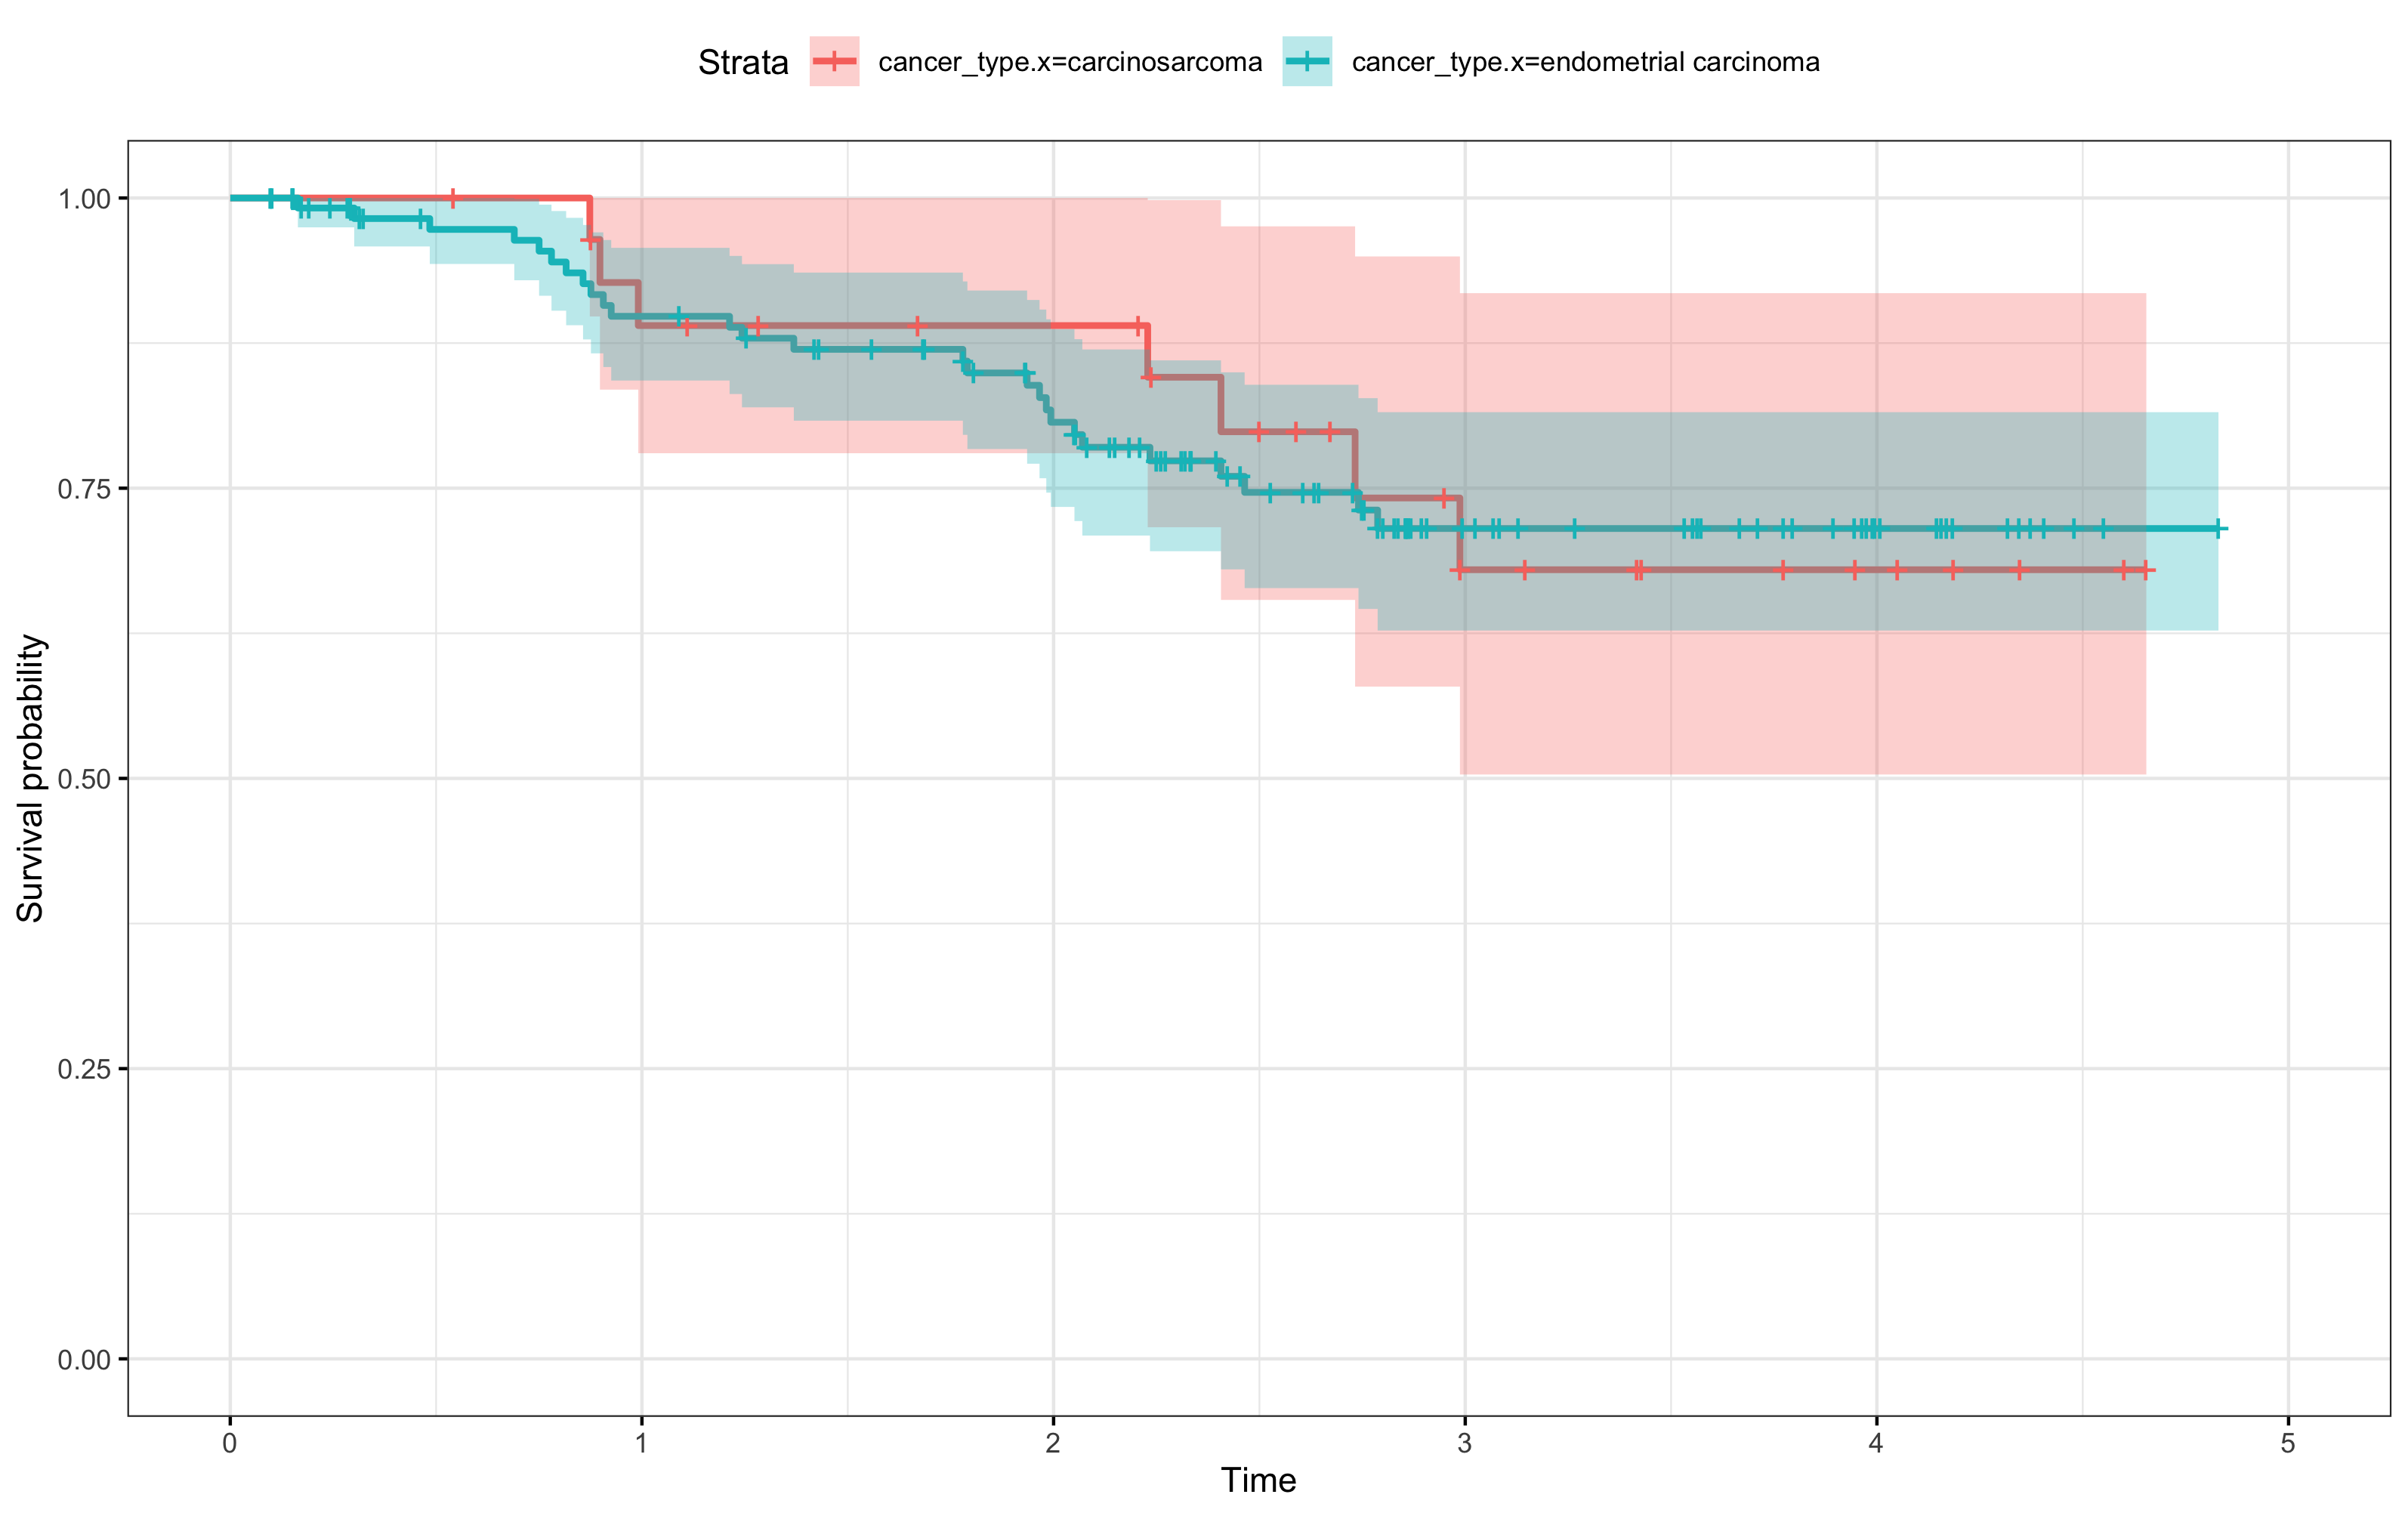
\includegraphics[width=3in]{cancertype.png}
    \caption{Step-wise survival curves estimated by the Breslow Estimator}
    \label{fig:fig3}   % label should change
    \end{figure}


\section{Competing Risks}

Understanding competing risks is now relatively intuitive as an extension of  the single-endpoint framework in terms of a multi-state model. A general survival model can be generalized to a competing risks setting by introducing several competing absorbing states, which represent the possible event types. In this setting, we can model the occurrence of a competing event as a transition into the corresponding competing event state. This model is depicted in \autoref{fig:fig4} for a finite number ($J$) competing risks. While this is theoretically possible under the competing risks framework, we only consider the simplest case ($J = 2$) in this work, which is also the most commonly collected type of competing risks data.


\begin{figure}[h]
    \centering
    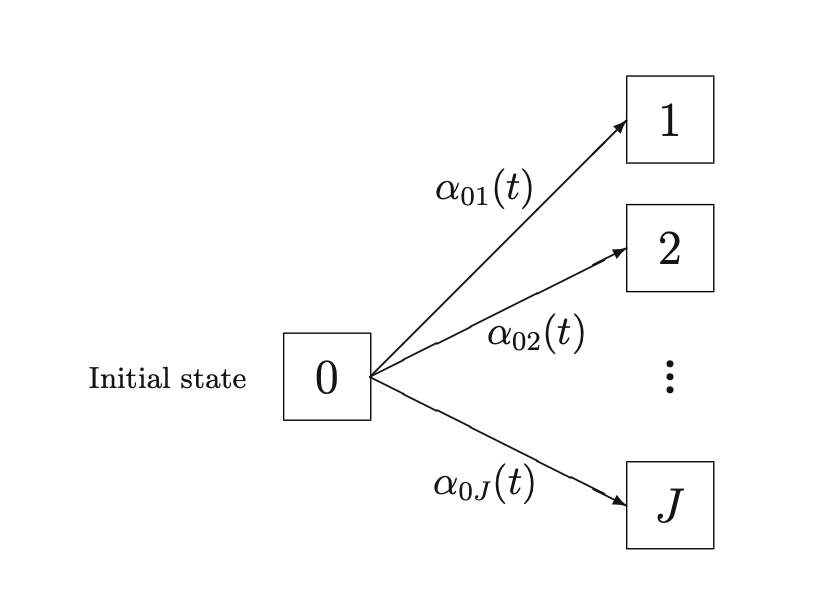
\includegraphics[width=3in]{competing_risks.png}
    \caption{Competing risks multistate model with cause-specific hazards $\alpha_{0j}(t), j = 1, 2, ....., J$. The vertical dots The vertical dots indicate the competing event states 
    $3, 4, ...., J-1$.}
    \label{fig:fig4}   % label should change
    \end{figure}

\begin{figure}[h]
    \centering
    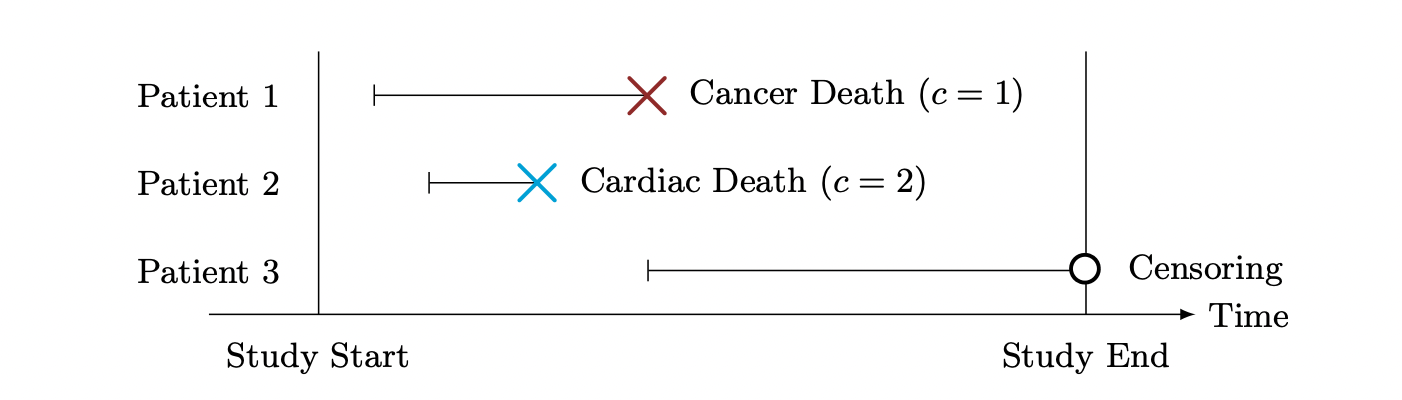
\includegraphics[width=6in]{competingrisks_example.png}
    \caption{Schematic of observation times for three example patients with competing risks}
    \label{fig:fig6}   % label should change
    \end{figure}

To look at an example (\autoref{fig:fig6}), when studying the survival of cancer patients, competing events can be cancer-related death $(c = 1)$, our primary cause of interest, or death by cardiac disease $(c = 2)$. An individual is no longer \textit{at risk} of cardiac disease once they have died of cancer, and vice versa, i.e they are mutually exclusive events.
We can use single end-point survival analysis, such as the Kaplan-Meier estimate to analyze competing risks data and estimate the survival function by recording other events as censored observations. However, the independent censoring assumption $(T \wedge C)$ does not hold in this setting: it may be unreasonable to assume that subjects who died of the competing risk (and were thus treated as censored) can be represented by those subjects who remained alive and had not yet died of any cause.  This can lead to biased estimates in standard survival models, as well as overestimation of the survival function.
\smallskip \par 
In recent years, the analysis of competing risks data has gained increasing prominence in various fields of study, but yet remains an area of survival analysis that has been relatively less-explored. As populations age and chronic diseases become more prevalent, the occurrence of multiple competing events, such as multiple types of diseases or comorbidities, has become a critical aspect of research. The availability of large-scale longitudinal datasets has facilitated need for the accurate analysis of competing risks. Thus, understanding and appropriately analyzing competing risks data is essential for accurate risk assessment, for identifying prognostic factors and for clinical decision-making, to accurately account for patients being \textit{at risk} for more than one comorbidity.

\subsection{Cause-specific Hazards}

Under competing risks, the hazard function translates to cause-specific hazards $\alpha_{0j}(t), j = 1, 2$, one for each event in a two-competing risks setting, of the form: 
\begin{equation}
A_{0j}(t) := \int_{0}^{t} \alpha_{0j} (u) du, j = 1, 2
\end{equation}

In a competing risks analysis, both cause-specific hazards (which can be thought of as "transition intensities") completely determine the stochastic behaviour of the competing risks process in the multistate model.

\subsection{Cumulative Incidence Function (CIF)}

As previously discussed, from the perspective of clinical patient care, the most relevant quantity is often estimating the long-term risk of experiencing a certain event given the patient’s particular characteristics. This is often of interest in the competing setting, and is captured by estimating the cumulative incidence function (CIF) or the absolute risk, i.e., the expected proportion of individuals experiencing a certain event over the course of time. The cumulative incidence function for each cause can be expressed as function of the cause-specific hazards and the survival function $P(T > u-)$ as shown below: 

\begin{equation}
    P(T \leq t) = \int^{t}_{0} P(T > u-) \alpha (u) du
\end{equation}

The cumulative incidence function was proposed to solve the inadequacy of the Kaplan-Meier estimate for competing risks data by estimating the marginal probability of an event of interest as a function of its cause-specific hazard and the overall survival probability. In the simple single-endpoint survival analysis setting, it breaks down to $1- \hat{S}(t)$, where $\hat{S}(t)$ is the Kaplan Meier estimate. 

\section{Regularization and Variable Selection for Survival Analysis}

TALK ABOUT HIGH-DIMENSIONAL DATASETS, NEED TO PREVENT OVERFITTING, IDENTIFY IMPORTANT GENES/BIOMARKERS

OVERVIEW OF ELASTIC NET FAMILY: FOCUS ON LASSO

\section{Regularized modelling approaches for competing risks}

TALK ABOUT CAUSE-SPECIFIC AND CIF MODELS DIFFERENCE 

MODELS TO TALK ABOUT: 

1) BOOSTED COX
2) PENALIZED FINE-GRAY
3) PENALIZED COX
4) DIRECT BINOMIAL

\section{Survival Analysis Model Performance Measures}

1) BRIER SCORE

2) TALK ABOUT SENS, SPEC, MCC

z\chapter{Case-base sampling for competing risks}
\label{ch:chpapter3}

In this chapter, we discuss the details of our proposed method: penalized case-base sampling. We provide an overview of the theory behind this sampling and connect this to the penalized multinomial parameterization.


\section{Case-base sampling}

\section{Multinomial parameterization}

\section{Regularization and optimization}

\chapter{Experiments}
\label{ch:experiments}

\section{Variable selection performance}
\section{Cumulative Incidence Function prediction performance}
\section{Bladder Cancer Dataset Analysis}
\chapter{Conclusions and Future Work}
\label{ch:conclusion}



%    2. Main body
% Generally recommended to put each chapter into a separate file
%\include{relatedwork}
%\include{model}
%\include{impl}
%\include{discussion}
%\include{conclusions}

%    3. Notes
%    4. Footnotes

%    5. Bibliography
\begin{singlespace}
\raggedright
\bibliographystyle{abbrvnat}
\bibliography{biblio}
\end{singlespace}

\appendix
%    6. Appendices (including copies of all required UBC Research
%       Ethics Board's Certificates of Approval)
%\include{reb-coa}	% pdfpages is useful here
\chapter{Supporting Materials}

This would be any supporting material not central to the dissertation.
For example:
\begin{itemize}
\item additional details of methodology and/or data;
\item diagrams of specialized equipment developed.;
\item copies of questionnaires and survey instruments.
\end{itemize}


\backmatter
%    7. Index
% See the makeindex package: the following page provides a quick overview
% <http://www.image.ufl.edu/help/latex/latex_indexes.shtml>


\end{document}
